\documentclass[10pt]{article}
\usepackage{amsmath} % for align environment
\usepackage{booktabs} % for better tables
\usepackage{minted}
\usepackage[utf8]{inputenc}
\usepackage[T1]{fontenc}
\usepackage{amsmath}
\usepackage{amsfonts}
\usepackage{amssymb}
\usepackage[version=4]{mhchem}
\usepackage{stmaryrd}
\usepackage{hyperref}
\hypersetup{colorlinks=true, linkcolor=blue, filecolor=magenta, urlcolor=cyan,}
\urlstyle{same}
\usepackage{bbold}
\usepackage{graphicx}
\usepackage[export]{adjustbox}
\graphicspath{ {./images/} }

\title{CM146, Winter 2024 
 Problem Set 2: Perceptron and Regression 
 Due February 16, 2024 at 11:59 pm }

\author{Harris Doan}
\date{February 15, 2024}


%New command to display footnote whose markers will always be hidden
\let\svthefootnote\thefootnote
\newcommand\blfootnotetext[1]{%
  \let\thefootnote\relax\footnote{#1}%
  \addtocounter{footnote}{-1}%
  \let\thefootnote\svthefootnote%
}

%Overriding the \footnotetext command to hide the marker if its value is `0`
\let\svfootnotetext\footnotetext
\renewcommand\footnotetext[2][?]{%
  \if\relax#1\relax%
    \ifnum\value{footnote}=0\blfootnotetext{#2}\else\svfootnotetext{#2}\fi%
  \else%
    \if?#1\ifnum\value{footnote}=0\blfootnotetext{#2}\else\svfootnotetext{#2}\fi%
    \else\svfootnotetext[#1]{#2}\fi%
  \fi
}

\begin{document}
\maketitle
\section*{Submission}
\begin{itemize}
  \item Submit your solutions electronically on the course Gradescope site as PDF files.
  \item If you plan to typeset your solutions, please use the LaTeX solution template. If you must submit scanned handwritten solutions, please use a black pen on blank white paper and a high-quality scanner app.
\end{itemize}

Parts of this assignment are adapted from course material by Andrew Ng (Stanford), Jenna Wiens (UMich) and Jessica Wu (Harvey Mudd).

\section*{1 Perceptron $[2 \mathrm{pts}]$}
Design (specify $\boldsymbol{\theta}$ for) a two-input perceptron (with an additional bias or offset term) that computes the following boolean functions. Assume $T=1$ and $F=-1$. If a valid perceptron exists, show that it is not unique by designing another valid perceptron (with a different hyperplane, not simply through normalization). If no perceptron exists, state why.
(a) (1 pts) OR
(b) (1 pts) XOR

\paragraph{1a Answer.) OR}
\hspace{1cm}

OR Truth Table:\\
\begin{tabular}{cc|c}
$x_1$ & $x_2$ & $x_1 \lor x_2$ \\ \hline
1 & 1 & 1 \\
1 & -1 & 1 \\
-1 & 1 & 1 \\
-1 & -1 & -1 \\
\end{tabular} \\

When graphed with $X_1$ on the horizontal axis and $X_2$ on the vertical axis,
points with a value of 1 are plotted in the first, second, and fourth quadrants.
Conversely, a point with a value of -1 is found in the third quadrant. It is possible
to draw a line that delineates the point with a value of -1 from those with a value of 1,
demonstrating that the data points can be separated linearly. Denoting $\theta$ as
$\theta = [w_0, w_1, w_2]^T$, it is shown that the values of $\theta$ that facilitate
this separation include $\theta = \left[\frac{3}{4}, 1, 1\right]^T$ and $\theta = \left[\frac{1}{2}, 1, 1\right]^T$.

\paragraph{1b Answer.) XOR}
\hspace{1cm}

XOR Truth Table:\\
\begin{tabular}{cc|c}
$x_1$ & $x_2$ & $x_1 \oplus x_2$ \\ \hline
1 & 1 & -1 \\
1 & -1 & 1 \\
-1 & 1 & 1 \\
-1 & -1 & -1 \\
\end{tabular}\\

Graphing this XOR truth table, it becomes apparent that no line can be drawn to segregate the data points with +1 and -1 values, indicating the absence of a perceptron. The derived equations are:

\[
\begin{aligned}
\theta_0 - \theta_1 - \theta_2 &\leq 0, \\
\theta_0 - \theta_1 + \theta_2 &\geq 0, \\
\theta_0 + \theta_1 - \theta_2 &\geq 0, \\
\theta_0 + \theta_1 + \theta_2 &\leq 0.
\end{aligned}
\]

Merging the first and fourth equations yields \(2\theta_0 \leq 0\), and combining the second and third equations yields \(2\theta_0 \geq 0\), thus presenting a system of equations with no feasible solution. So therefore no valid perceptron exists.



\section*{2 Logistic Regression [10 pts]}
Consider the objective function that we minimize in logistic regression:

$$
J(\boldsymbol{\theta})=-\sum_{n=1}^{N}\left[y_{n} \log h_{\boldsymbol{\theta}}\left(\boldsymbol{x}_{n}\right)+\left(1-y_{n}\right) \log \left(1-h_{\boldsymbol{\theta}}\left(\boldsymbol{x}_{n}\right)\right)\right]
$$

where $h_{\boldsymbol{\theta}}(\boldsymbol{x})=\sigma\left(\boldsymbol{\theta}^{T} \boldsymbol{x}\right)=\frac{1}{1+e^{-\boldsymbol{\theta}^{T} \boldsymbol{x}}}$.

(a) (2 pts) Find the partial derivatives $\frac{\partial J}{\partial \theta_{j}}$.

\paragraph{2a Answer.) Finding the Partial Derivatives $\frac{\partial J}{\partial \theta_j}$:}
\hspace{1 cm}

The logistic function $h_{\theta}(x)$ is given by:
\[ h_{\theta}(x) = \sigma(\theta^T x) = \frac{1}{1+e^{-\theta^T x}}. \]

The derivative of $h_{\theta}(x)$ with respect to $\theta_j$ is given by the chain rule:
\[ \frac{\partial}{\partial \theta_j} h_{\theta}(x) = h_{\theta}(x)(1 - h_{\theta}(x))x_j. \]

Using this, the partial derivative of $J(\theta)$ with respect to $\theta_j$ is:
\[ \frac{\partial J}{\partial \theta_j} = -\sum_{n=1}^{N} \left[ y_n \frac{1}{h_{\theta}(x_n)} - (1 - y_n) \frac{1}{1 - h_{\theta}(x_n)} \right] \frac{\partial}{\partial \theta_j} h_{\theta}(x_n) \]
\[ \frac{\partial J}{\partial \theta_j} = -\sum_{n=1}^{N} \left[ y_n (1 - h_{\theta}(x_n)) - (1 - y_n) h_{\theta}(x_n) \right] x_{n,j} \]
\[ \frac{\partial J}{\partial \theta_j} = \sum_{n=1}^{N} \left[ h_{\theta}(x_n) - y_n \right] x_{n,j}. \]


(b) (3 pts) Find the partial second derivatives $\frac{\partial^{2} J}{\partial \theta_{j} \partial \theta_{k}}$ and show that the Hessian (the matrix $\boldsymbol{H}$ of second derivatives with elements $\left.H_{j k}=\frac{\partial^{2} J}{\partial \theta_{j} \partial \theta_{k}}\right)$ can be written as $\boldsymbol{H}=\sum_{n=1}^{N} h_{\boldsymbol{\theta}}\left(\boldsymbol{x}_{n}\right)\left(1-h_{\boldsymbol{\theta}}\left(\boldsymbol{x}_{n}\right)\right) \boldsymbol{x}_{n} \boldsymbol{x}_{n}^{T}$.

\paragraph{2b Answer.) Finding the Partial Second Derivatives and the Hessian $H$:}
\hspace{1 cm}

To find the second derivative, we differentiate the first derivative with respect to $\theta_k$:
\[ \frac{\partial^2 J}{\partial \theta_j \partial \theta_k} = \frac{\partial}{\partial \theta_k} \left( \frac{\partial J}{\partial \theta_j} \right) \]
\[ \frac{\partial^2 J}{\partial \theta_j \partial \theta_k} = \sum_{n=1}^{N} h_{\theta}(x_n)(1 - h_{\theta}(x_n)) x_{n,j} x_{n,k}. \]

The Hessian matrix $H$ has elements $H_{jk}$ given by:
\[ H_{jk} = \frac{\partial^2 J}{\partial \theta_j \partial \theta_k} = \sum_{n=1}^{N} h_{\theta}(x_n)(1 - h_{\theta}(x_n)) x_{n,j} x_{n,k}. \]


(c) (5 pts) Show that $J$ is a convex function and therefore has no local minima other than the global one.

Hint: A function $J$ is convex if its Hessian is positive semi-definite (PSD), written $\boldsymbol{H} \succeq 0$. A matrix is PSD if and only if

$$
\boldsymbol{z}^{T} \boldsymbol{H} \boldsymbol{z} \equiv \sum_{j, k} z_{j} z_{k} H_{j k} \geq 0
$$

for all real vectors $\boldsymbol{z}$.

\paragraph{2c Answer.) Showing that $J$ is Convex:}
\hspace{1 cm}

A function is convex if its Hessian is positive semi-definite (PSD), which means for any vector $z$, the following condition holds:
\[ z^T H z = \sum_{j,k} z_j z_k H_{jk} \geq 0 \]

For the logistic regression cost function, each element $H_{jk}$ is non-negative because $h_{\theta}(x_n)(1 - h_{\theta}(x_n))$ is always non-negative as it is a product of probabilities. Therefore, the sum $\sum_{j,k} z_j z_k H_{jk}$ is also non-negative, implying that $H$ is PSD and $J(\theta)$ is convex.


\section*{3 Maximum Likelihood Estimation [15 pts]}
Suppose we observe the values of $n$ independent random variables $X_{1}, \ldots, X_{n}$ drawn from the same Bernoulli distribution with parameter $\theta^{1}$. In other words, for each $X_{i}$, we know that

$$
P\left(X_{i}=1\right)=\theta \quad \text { and } \quad P\left(X_{i}=0\right)=1-\theta \text {. }
$$

Our goal is to estimate the value of $\theta$ from these observed values of $X_{1}$ through $X_{n}$.

For any hypothetical value $\hat{\theta}$, we can compute the probability of observing the outcome $X_{1}, \ldots, X_{n}$ if the true parameter value $\theta$ were equal to $\hat{\theta}$. This probability of the observed data is often called the likelihood, and the function $L(\theta)$ that maps each $\theta$ to the corresponding likelihood is called the likelihood function. A natural way to estimate the unknown parameter $\theta$ is to choose the $\theta$ that maximizes the likelihood function. Formally,

$$
\hat{\theta}_{M L E}=\underset{\theta}{\arg \max } L(\theta) .
$$

(a) (3 pts) Write a formula for the likelihood function, $L(\theta)=P\left(X_{1}, \ldots, X_{n} ; \theta\right)$. Your function should depend on the random variables $X_{1}, \ldots, X_{n}$ and the hypothetical parameter $\theta$. Does the likelihood function depend on the order in which the random variables are observed?

\paragraph{ 3a Answer.) Likelihood }
\hspace{1cm}
In the case of a Bernoulli distribution, under the assumption that the samples are independent and identically distributed (IID), the likelihood function is given by the product of the probabilities for each observation:

\[ L(\theta) = \prod_{i=1}^{n} P(x_i; \theta) \]

This is further detailed as the product of the probability of each individual outcome, parameterized by \(\theta\), which is:

\[ L(\theta) = \prod_{i=1}^{n} \theta^{x_i} (1 - \theta)^{1 - x_i} \]

Due to the IID assumption, the order of observation of the random variables does not affect the form of the likelihood function.


(b) (6 pts) Since the log function is increasing, the $\theta$ that maximizes the log likelihood $\ell(\theta)=$ $\log (L(\theta))$ is the same as the $\theta$ that maximizes the likelihood. Find $\ell(\theta)$ and its first and second derivatives, and use these to find a closed-form formula for the MLE. For this part, assume we use the natural logarithm (i.e. logarithm base $e$ ).

\paragraph{ 3b Answer.) Derivatives and MLE}
\hspace{1cm}

To extract the log-likelihood from the likelihood of a Bernoulli distributed set of observations, we take the natural logarithm of the product of probabilities, converting it into a sum of logarithms due to the logarithmic property that converts products into sums. The log-likelihood, denoted as \( l(\theta) \), is expressed as:

\[ l(\theta) = \log \left( \prod_{i=1}^{N} P(x_i; \theta) \right) = \sum_{i=1}^{N} \log P(x_i; \theta) = \sum_{i=1}^{N} \left[ x_i \log \theta + (1 - x_i) \log(1 - \theta) \right] \]

For maximization, we proceed by taking the derivative of the log-likelihood with respect to \( \theta \) and setting it to zero to solve for \( \theta \). The derivative is given by:

\[ \frac{dl}{d\theta} = \sum_{i=1}^{N} \left[ \frac{x_i}{\theta} - \frac{1 - x_i}{1 - \theta} \right] \]

Further, the second derivative is taken to ensure the concavity of the log-likelihood function, which is necessary for the existence of a maximum point:

\[ \frac{d^2l}{d\theta^2} = \sum_{i=1}^{N} \left[ -\frac{x_i}{\theta^2} - \frac{1 - x_i}{(1 - \theta)^2} \right] \]

To find the maximum likelihood estimate of \( \theta \), we equate the first derivative to zero. If we let the sum of all \( x_i \) be \( x_{\text{total}} \), the solution for \( \theta \) is:

\[ \theta = \frac{x_{\text{total}}}{N} = \bar{x} \]

This indicates that the maximum likelihood estimator for \( \theta \) in a Bernoulli distribution is simply the sample mean.\\


(c) (3 pts) Suppose that $n=10$ and the data set contains six $1 \mathrm{~s}$ and four 0s. Write a short program \href{http://likelihood.py}{likelihood.py} that plots the likelihood function of this data for each value of $\theta$ in $\{0,0.01,0.02, \ldots, 1.0\}$ (use np.linspace ( $\ldots$ ) to generate this spacing). For the plot, the $\mathrm{x}$-axis should be $\theta$ and the $\mathrm{y}$-axis $L(\theta)$. Scale your $\mathrm{y}$-axis so that you can see some variation in its value. Include the plot in your writeup (there is no need to submit your code). Estimate $\hat{\theta}_{M L E}$ by marking on the x-axis the value of $\theta$ that maximizes the likelihood. Does the answer agree with the closed form answer?

\paragraph{3c Answer.) Likelihood of $\theta$ Plotted onto a Graph}
\hspace{1cm}

To determine the value of \( \theta \) that maximizes the likelihood function, we plot the likelihood as a function of \( \theta \) and observe where it reaches its peak. The plot below visualizes the likelihood function derived from the Bernoulli distribution for a range of \( \theta \) values from 0 to 1.

\begin{figure}[h!]
  \centering
  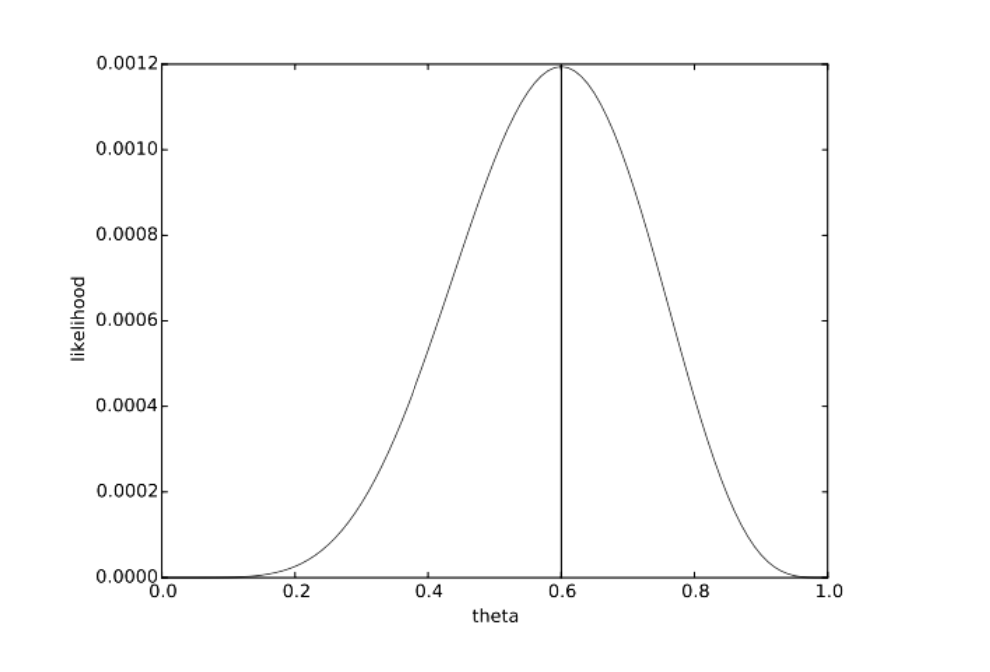
\includegraphics[width=0.8\textwidth]{image.png} % Make sure to have the correct path to the image
  \caption{The likelihood function of \( \theta \).}
\end{figure}

The value of \( \theta \) that appears to maximize the likelihood is 0.6. This result is consistent with the outcome obtained from solving the first derivative of the log-likelihood function set to zero, as shown in section 3(b).

(d) (3 pts) Create three more likelihood plots: one where $n=5$ and the data set contains three $1 \mathrm{~s}$ and two 0s; one where $n=100$ and the data set contains sixty $1 \mathrm{~s}$ and forty $0 \mathrm{~s}$; and one where $n=10$ and there are five 1 s and five 0s. Include these plots in your writeup, and describe how the likelihood functions and maximum likelihood estimates compare for the different data sets.
\footnotetext{${ }^{1}$ This is a common assumption for sampling data. So we will denote this assumption as iid, short for Independent and Identically Distributed, meaning that each random variable has the same distribution and is drawn independent of all the other random variables
}

\paragraph{3d Answer.) More Plots}
\hspace{1cm}

For a series of Bernoulli trials, the likelihood function for \( \theta \) can be visualized by plotting the function across different values of \( \theta \). Below are three different scenarios based on the number of trials and the number of successes (1s) observed.

\subsection*{For \( n = 5 \) with three 1s and two 0s:}
\begin{figure}[h!]
  \centering
  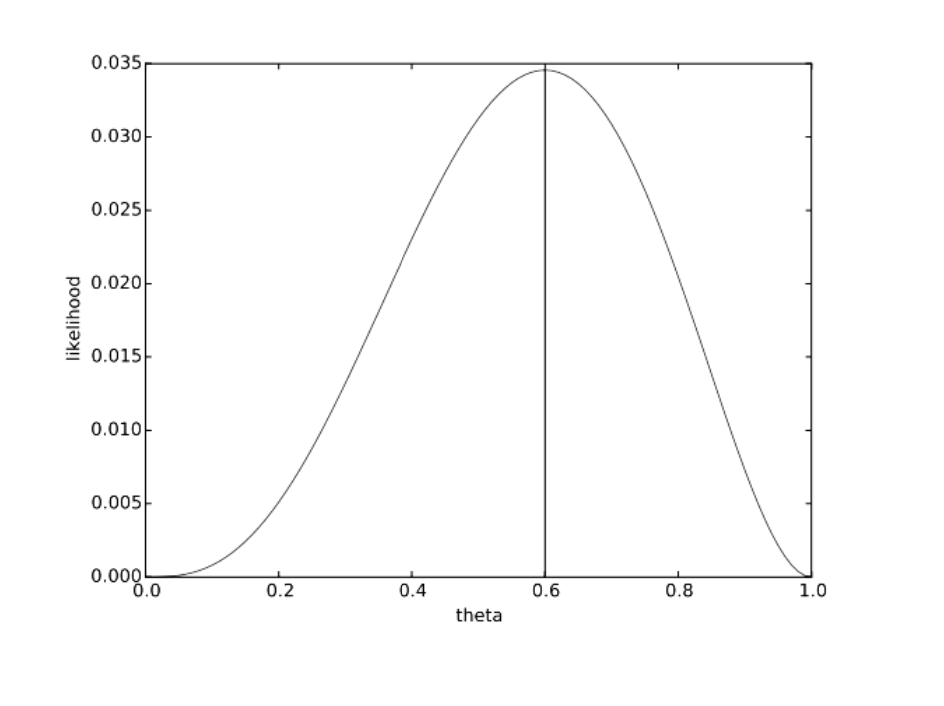
\includegraphics[width=0.8\textwidth]{image1.png}
  \caption{Likelihood function for \( n = 5 \) with three 1s and two 0s.}
\end{figure}

The graph is centered at \( \theta = 0.6 \), consistent with the proportion of successes. Due to a smaller sample size, the standard deviation is larger, indicating a wider spread in the likelihood estimates.

\subsection*{For \( n = 100 \) with sixty 1s and forty 0s:}
\begin{figure}[h!]
  \centering
  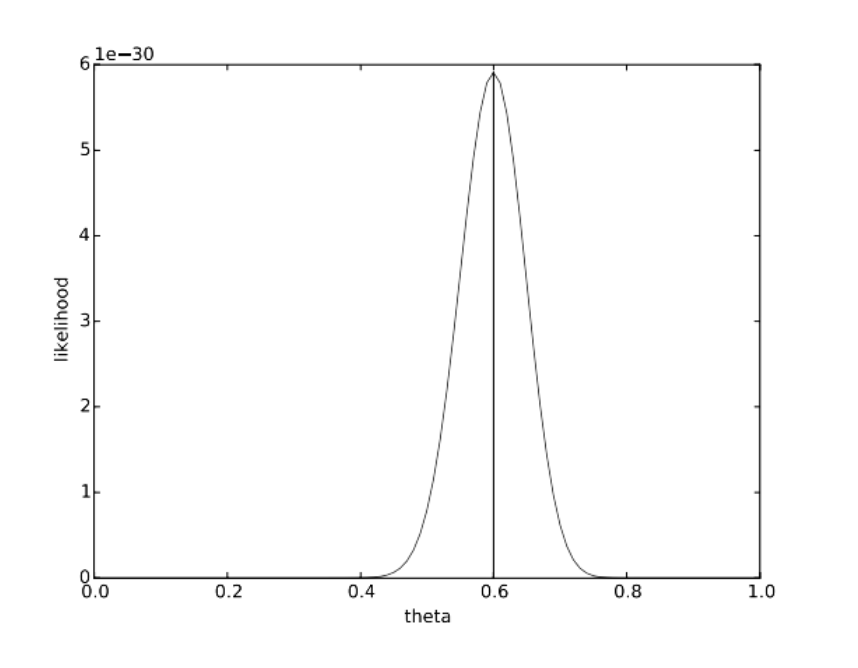
\includegraphics[width=0.8\textwidth]{image2.png}
  \caption{Likelihood function for \( n = 100 \) with sixty 1s and forty 0s.}
\end{figure}

With \( n = 100 \), the graph remains centered at \( \theta = 0.6 \) but becomes narrower, reflecting a lower standard deviation as per the central limit theorem. The peak of the likelihood is significantly lower due to the increased sample size.

\subsection*{For \( n = 10 \) with five 1s and five 0s:}
\begin{figure}[h!]
  \centering
  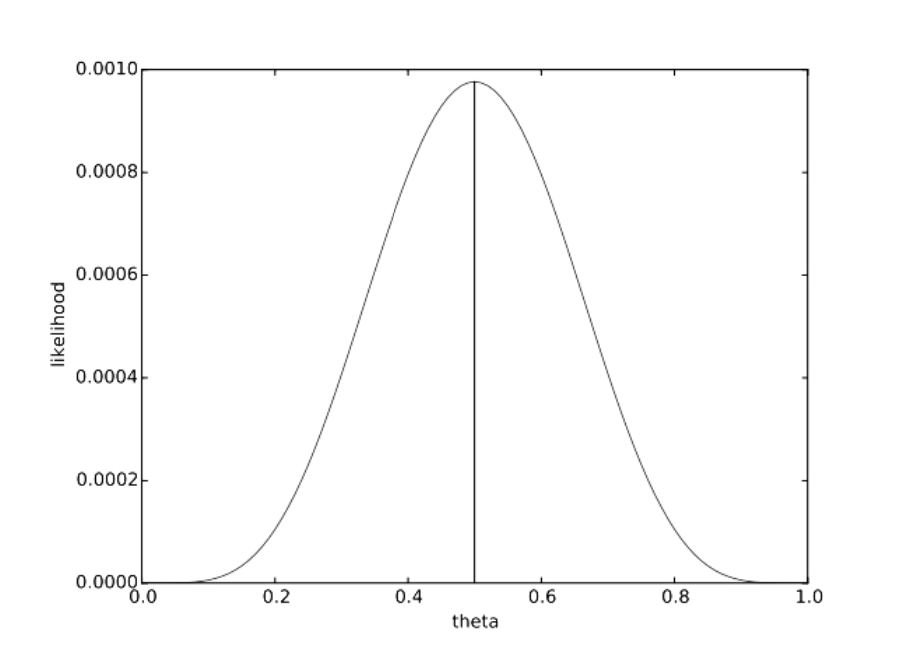
\includegraphics[width=0.8\textwidth]{image3.png}
  \caption{Likelihood function for \( n = 10 \) with five 1s and five 0s.}
\end{figure}

In this case, the graph is centered at \( \theta = 0.5 \), reflecting an equal number of successes and failures. The spread is similar to the first scenario, and the maximum likelihood value is comparable to the \( n = 10 \) case. As the number of trials \( n \) varies, there is a noticeable effect on the standard deviation of the likelihood function. Larger \( n \) results in a more peaked likelihood function, with the graph centering around the proportion of successes. This behavior illustrates the central limit theorem in action, where the distribution of the sample mean (or in this case, the sample proportion) becomes increasingly normal as \( n \) increases.


\section*{4 Implementation: Polynomial Regression [20 pts]}
In this exercise, you will work through linear and polynomial regression. Our data consists of inputs $x_{n} \in \mathbb{R}$ and outputs $y_{n} \in \mathbb{R}, n \in\{1, \ldots, N\}$, which are related through a target function $y=f(x)$. Your goal is to learn a linear predictor $h_{\boldsymbol{\theta}}(x)$ that best approximates $f(x)$. But this time, rather than using scikit-learn, we will further open the "black-box", and you will implement the regression model!

code and data

\begin{itemize}
  \item code: CS146\_Winter2024\_PS2.ipynb
  \item data: regression\_train.csv, regression\_test.csv
\end{itemize}

Similar to PS1, copy the colab notebook to your drive and make the changes to the notebook. Mount the drive appropriately and copy the data to your drive to access via colab.

The notebook has marked blocks where you need to code.

$\# \# \#=========T O D O: S T A R T=========\# \# \#$

$\# \# \#=========T O D O: E N D==========\# \# \#$

Note: For parts b, c, g, and h (and only these parts), you are expected to copypaste/screenshot your code snippet as a part of the solution in the submission pdf. Tip: If you are using $\mathrm{HT}_{\mathbf{E}} \mathrm{X}$, check out the Minted package (example) for code highlighting.

This is likely the first time that many of you are working with numpy and matrix operations within a programming environment. For the uninitiated, you may find it useful to work through a numpy tutorial first. ${ }^{2}$ Here are some things to keep in mind as you complete this problem:
- If you are seeing many errors at runtime, inspect your matrix operations to make sure that you are adding and multiplying matrices of compatible dimensions. Printing the dimensions of variables with the $\mathrm{X}$. shape command will help you debug.
- When working with numpy arrays, remember that numpy interprets the $*$ operator as elementwise multiplication. This is a common source of size incompatibility errors. If you want matrix multiplication, you need to use the dot function in Python. For example, $A * B$ does element-wise multiplication while $\operatorname{dot}(A, B)$ does a matrix multiply.
- Be careful when handling numpy vectors (rank-1 arrays): the vector shapes $1 \times N, N \times$ 1 , and $N$ are all different things. For these dimensions, we follow the the conventions of scikit-learn's LinearRegression class ${ }^{3}$. Most importantly, unless otherwise indicated (in the code documentation), both column and row vectors are rank- 1 arrays of shape $N$, not rank- 2 arrays of shape $N \times 1$ or shape $1 \times N$.
\footnotetext{${ }^{2}$ Try out SciPy's tutorial (\href{https://numpy.org/doc/stable/user/quickstart.html}{https://numpy.org/doc/stable/user/quickstart.html}), or use your favorite search engine to find an alternative. Those familiar with Matlab may find the "Numpy for Matlab Users" documentation (\href{https://numpy.org/doc/stable/user/numpy-for-matlab-users.html}{https://numpy.org/doc/stable/user/numpy-for-matlab-users.html}) more helpful.

${ }^{3}$ \href{http://scikit-learn.org/stable/modules/generated/sklearn.linear_model.LinearRegression.html}{http://scikit-learn.org/stable/modules/generated/sklearn.linear\_model.LinearRegression.html}
}

\section*{Visualization [1 pts]}
It is often useful to understand the data through visualizations. For this data set, you can use a scatter plot to visualize the data since it has only two properties to plot ( $x$ and $y$ ).

(a) (1 pts) Visualize the training and test data using the plot\_data(...) function. What do you observe? For example, can you make an educated guess on the effectiveness of linear regression in predicting the data?

\paragraph{4a Answer.) Visualization}
\hspace{1cm}

\begin{figure}[h!]
  \centering
  \begin{minipage}[b]{0.45\textwidth}
    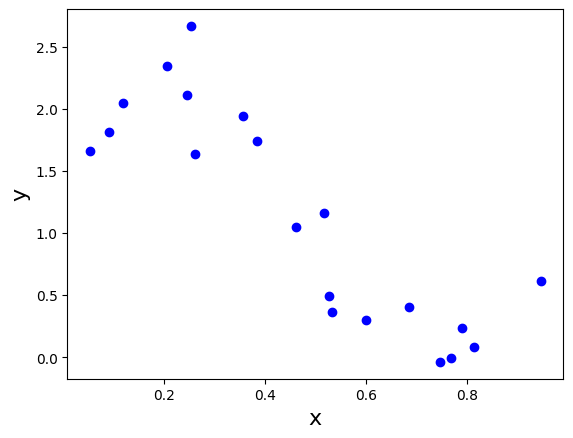
\includegraphics[width=\textwidth]{train_data.png}
    \caption{Training Data}
  \end{minipage}
  \hfill
  \begin{minipage}[b]{0.45\textwidth}
    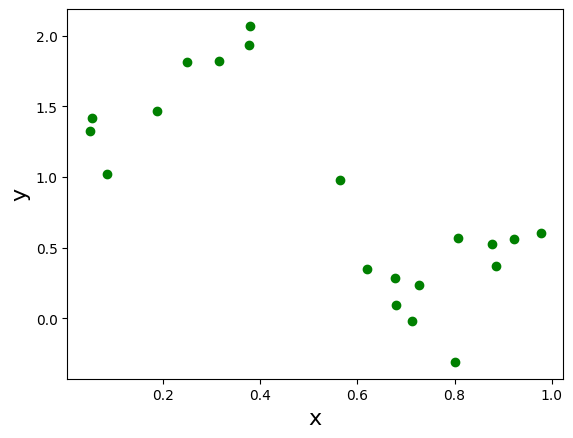
\includegraphics[width=\textwidth]{test_data.png}
    \caption{Test Data}
  \end{minipage}
\end{figure}

The training dataset exhibits a mild negative correlation between X and y, with a noticeable amount of noise present. Conversely, the test dataset displays a significantly higher level of noise, suggesting that a polynomial regression model could potentially provide a better fit for the test data compared to a linear regression model. The graphics presented sequentially illustrate the characteristics of the training and test datasets, respectively.\\

\section*{Linear Regression [12 pts]}
Recall that linear regression attempts to minimize the objective function

$$
J(\boldsymbol{\theta})=\sum_{n=1}^{N}\left(h_{\boldsymbol{\theta}}\left(\boldsymbol{x}_{n}\right)-y_{n}\right)^{2}
$$

In this problem, we will use the matrix-vector form where

$$
\boldsymbol{y}=\left(\begin{array}{c}
y_{1} \\
y_{2} \\
\vdots \\
y_{N}
\end{array}\right), \quad \boldsymbol{X}=\left(\begin{array}{c}
\boldsymbol{x}_{1}^{T} \\
\boldsymbol{x}_{2}^{T} \\
\vdots \\
\boldsymbol{x}_{N}^{T}
\end{array}\right), \quad \boldsymbol{\theta}=\left(\begin{array}{c}
\theta_{0} \\
\theta_{1} \\
\theta_{2} \\
\vdots \\
\theta_{D}
\end{array}\right)
$$

and each instance $\boldsymbol{x}_{n}=\left(1, x_{n, 1}, \ldots, x_{n, D}\right)^{T}$.

In this instance, the number of input features $D=1$.

Rather than working with this fully generalized, multivariate case, let us start by considering a simple linear regression model:

$$
h_{\boldsymbol{\theta}}(\boldsymbol{x})=\boldsymbol{\theta}^{T} \boldsymbol{x}=\theta_{0}+\theta_{1} x_{1}
$$

The Colab notebook contains the skeleton code for the class PolynomialRegression. Objects of this class can be instantiated as model $=$ PolynomialRegression ( $\mathrm{m}$ ) where $m$ is the degree of the polynomial feature vector where the feature vector for instance $n$ is $\left(1, x_{n, 1}, x_{n, 1}^{2}, \ldots, x_{n, 1}^{m}\right)^{T}$. Setting $m=1$ instantiates an object where the feature vector for instance $n$ is $\left(1, x_{n, 1}\right)^{T}$.

(b) (1 pts) Note that to take into account the intercept term $\left(\theta_{0}\right)$, we can add an additional "feature" to each instance and set it to one, e.g. $x_{n, 0}=1$. This is equivalent to adding an additional first column to $\boldsymbol{X}$ and setting it to all ones.

\paragraph{4b Answer.) Intercept}
\hspace{1cm}

Code: \\
\begin{minted}{python}
        ### ========== TODO : START ========== ###
        # part b: modify to create matrix for simple linear model
        X = np.append(np.ones([n,1]), X, 1)
        ### ========== TODO : END ========== ###
\end{minted}

Modify PolynomialRegression.generate\_polynomial\_features (.. . ) to create the matrix $\boldsymbol{X}$ for a simple linear model. Copy-paste/screenshot your code snippet.\\

(c) (1 pts) Before tackling the harder problem of training the regression model, complete PolynomialRegression.predict(...) to predict $\boldsymbol{y}$ from $\boldsymbol{X}$ and $\boldsymbol{\theta}$. Copy-paste/screenshot your code snippet.


\paragraph{4c Answer.) Polynomial Regression}
\hspace{1cm}

Code: \\
\begin{minted}{python}
        ### ========== TODO : START ========== ###
        # part c: predict y
        y = np.dot(X, np.transpose(self.coef_))
        ### ========== TODO : END ========== ###
\end{minted}

(d) (5 pts) One way to solve linear regression is through gradient descent (GD).
Recall that the parameters of our model are the $\theta_{j}$ values. These are the values we will adjust to minimize $J(\boldsymbol{\theta})$.

$$
J(\boldsymbol{\theta})=\sum_{n=1}^{N}\left(h_{\boldsymbol{\theta}}\left(\boldsymbol{x}_{n}\right)-y_{n}\right)^{2}
$$

In gradient descent, each iteration performs the update

$$
\left.\theta_{j} \leftarrow \theta_{j}-2 \eta \sum_{n=1}^{N}\left(h_{\boldsymbol{\theta}}\left(\boldsymbol{x}_{n}\right)-y_{n}\right) x_{n, j} \quad \text { (simultaneously update } \theta_{j} \text { for all } j\right) .
$$

With each step of gradient descent, we expect our updated parameters $\theta_{j}$ to come closer to the parameters that will achieve the lowest value of $J(\boldsymbol{\theta})$.

\begin{itemize}
  \item As we perform gradient descent, it is helpful to monitor the convergence by computing the cost, i.e., the value of the objective function $J$. Complete PolynomialRegression. cost (. . ) to calculate $J(\boldsymbol{\theta})$.
\end{itemize}

If you have implemented everything correctly, then the following code snippet should return 40.234 .

\begin{center}
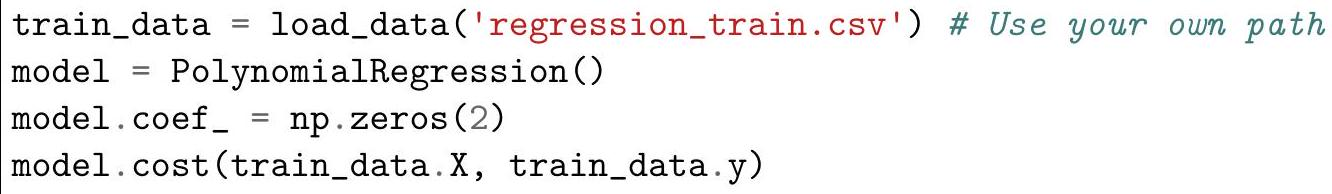
\includegraphics[max width=\textwidth]{2024_02_15_81352c3b436fa7594d79g-6}
\end{center}

\begin{itemize}
  \item Next, implement the gradient descent step in PolynomialRegression.fit\_GD(...). The loop structure has been written for you, and you only need to supply the updates to $\boldsymbol{\theta}$ and the new predictions $\hat{y}=h_{\boldsymbol{\theta}}(\boldsymbol{x})$ within each iteration.
\end{itemize}

We will use the following specifications for the gradient descent algorithm:

\begin{itemize}
  \item We run the algorithm for 10,000 iterations.
  \item We terminate the algorithm earlier if the value of the objective function is unchanged across consecutive iterations.
  \item We will use a fixed learning rate.
  \item Experiment with different values of learning rate $\eta=10^{-4}, 10^{-3}, 10^{-2}, 0.1$, and make a table of the coefficients, number of iterations until convergence (this number will be 10,000 if the algorithm did not converge in a smaller number of iterations) and the final value of the objective function. How do the coefficients compare? How quickly does each algorithm converge?
\end{itemize}\\

\paragraph{4d Answer.) Gradient Descent}
\hspace{1cm}

Code:\\
\begin{minted}{python}
            ### ========== TODO : START ========== ###
            # part d: update theta (self.coef_) using one step of GD
            # hint: you can write simultaneously update all w using vector math
            weights = np.array(list(self.coef_))
            for i, val in enumerate(self.coef_):
              total = 0
              for j, x in enumerate(X):
                total += (np.dot(weights, x) - y[j]) * x[i]
              self.coef_[i] += (-2) * eta * total

            # track error
            # hint: you cannot use self.predict(...) to make the predictions
            y_pred = np.dot(X, np.transpose(self.coef_))  # change this line
            err_list[t] = np.sum(np.power(y - y_pred, 2)) / float(n)
            ### ========== TODO : END ========== ###
\end{minted}

The following results were obtained after running the code:

\begin{table}[h!]
\centering
\begin{tabular}{@{}cccc@{}}
\toprule
Number of Iterations & Step Size ($\eta$) & [$\theta_0$, $\theta_1$] & Model Cost \\ \midrule
10,000               & $1 \times 10^{-1}$     & [Nan, NaN]    & NaN   \\
764               & $1 \times 10^{-2}$     & [2.44641, -2.81635]   & 3.912576  \\
7,020                & $1 \times 10^{-3}$     & [2.44641, -2.81635]      & 3.912576  \\
10,000                  & $1 \times 10^{-4}$ & [2.27045, -2.46068]   & 4.0864    \\ \bottomrule
\end{tabular}
\end{table}

The analysis reveals that a step size approximately equal to $10^{-2}$ yields the most favorable outcomes, effectively balancing efficiency and convergence within the span of 10,000 iterations. Notably, a step size of $10^{-3}$, while still within an acceptable range, manifests as slightly less efficient due to marginally slower convergence rates. Contrarily, a step size of $10^{-4}$, despite falling within the permissible iteration threshold, is deemed too conservative, extending the time required for convergence. In contrast, a step size of 0.1 surpasses the optimal threshold, reaching the iteration limit prematurely and exhibiting significant divergence from expected coefficient values, indicative of numerical instability. Specifically, with a step size of $10^{-3}$, the coefficient vector converges closely to the results obtained with $10^{-2}$. However, the convergence trajectory for $10^{-4}$, albeit gradual, suggests potential alignment with the $10^{-2}$ results if granted a higher iteration allowance. Conversely, for a step size of 0.1, the convergence is not only non-existent but also suggests a propensity for computational instability.\\

(e) (4 pts) In class, we learned that the closed-form solution to linear regression is

$$
\boldsymbol{\theta}=\left(\boldsymbol{X}^{T} \boldsymbol{X}\right)^{-1} \boldsymbol{X}^{T} \boldsymbol{y}
$$

Using this formula, you will get an exact solution in one calculation: there is no "loop until convergence" like in gradient descent.

\begin{itemize}
  \item Implement the closed-form solution PolynomialRegression.fit(...).
  \item What is the closed-form solution coefficients? How do the coefficients and the cost compare to those obtained by GD? Use the 'time' module to compare its runtime to GD.
\end{itemize}

\paragraph{4e Answer.) Closed Form}
\hspace{1cm}

Code:\\
\begin{minted}{python}
        ### ========== TODO : START ========== ###
        # part e: implement closed-form solution
            xt_x = np.dot(np.transpose(X),X)
            self.coef_ = np.dot(np.dot(np.linalg.pinv(xt_x),np.transpose(X)),y)
            return self
        ### ========== TODO : END ========== ###
\end{minted}


The analytical solution, characterized by the closed-form expression, produces coefficients \(\theta_0 = 2.446407\) and \(\theta_1 = -2.816353\), with an ensuing cost of \(3.912576\). Relative to the iterative gradient descent method with fine-tuned step sizes, this direct calculation method not only yields more precise coefficients but also excels in computational speed, taking just \(0.00117\) seconds to complete—significantly faster than the \(0.12098\) seconds required for the gradient descent approach.\\


(f) (1 pts) Finally, set a learning rate $\eta$ for GD that is a function of $k$ (the number of iterations) (use $\eta_{k}=\frac{1}{1+k}$ ) and converges to the same solution yielded by the closed-form optimization (minus possible rounding errors). Update PolynomialRegression.fit\_GD(...) with your proposed learning rate. How many iterations does it take the algorithm to converge with your proposed learning rate?

\paragraph{4f Answer.) Auto Learning Rate}
\hspace{1cm}

\begin{minted}{python}
            ### ========== TODO : START ========== ###
            # part f: update step size
            # change the default eta in the function signature to 'eta=None'
            # and update the line below to your learning rate function
            if eta_input is None:
                n = tmax
                eta = 1/(1+n)  # change this line
            else:
                eta = eta_input
            ### ========== TODO : END ========== ###
\end{minted}

Adopting a dynamic step size strategy, the execution time is reduced to 0.068s, culminating in the algorithm's convergence at 1511 iterations to coefficient values of \(\theta_0 = 2.44641\) and \(\theta_1 = -2.81635\), aligning with the results from part (d) (rounded to five decimal places). The cost metric remains consistent as well. With an increasing number of iterations, there is a corresponding decrease in step size, allowing the algorithm to initially advance rapidly towards the minimum and then fine-tune the convergence by reducing the step size as it approaches the target.\\

\section*{Polynomial Regression [7 pts]}
Now let us consider the more complicated case of polynomial regression, where our hypothesis is

$$
h_{\boldsymbol{\theta}}(\boldsymbol{x})=\boldsymbol{\theta}^{T} \phi(\boldsymbol{x})=\theta_{0}+\theta_{1} x+\theta_{2} x^{2}+\ldots+\theta_{m} x^{m} .
$$

(g) (1 pts) Recall that polynomial regression can be considered as an extension of linear regression in which we replace our input matrix $\boldsymbol{X}$ with

$$
\boldsymbol{\Phi}=\left(\begin{array}{c}
\phi\left(x_{1}\right)^{T} \\
\phi\left(x_{2}\right)^{T} \\
\vdots \\
\phi\left(x_{N}\right)^{T}
\end{array}\right)
$$

where $\phi(x)$ is a function such that $\phi_{j}(x)=x^{j}$ for $j=0, \ldots, m$.

Update PolynomialRegression.generate\_polynomial\_features(...) to create an $m+1$ dimensional feature vector for each instance. Copy-paste/screenshot your code snippet.

\paragraph{4g Answer.) Polynomial Regression}
\hspace{1cm}

Code:\\
\begin{minted}{python}
        ### ========== TODO : START ========== ###
        # part g: modify to create matrix for polynomial model
        m = self.m_
        Phi = np.ones([n,1])
        for i in range(1, m + 1):
          Phi = np.append(Phi, X ** i, 1)
        ### ========== TODO : END ========== ###
\end{minted}

(h) (2 pts) Given $N$ training instances, it is always possible to obtain a "perfect fit" (a fit in which all the data points are exactly predicted) by setting the degree of the regression to $N-1$. Of course, we would expect such a fit to generalize poorly. In the remainder of this problem, you will investigate the problem of overfitting as a function of the degree of the polynomial, $m$. To measure overfitting, we will use the Root-Mean-Square (RMS) error, defined as

$$
E_{R M S}=\sqrt{J(\boldsymbol{\theta}) / N}
$$

where $N$ is the number of instances. ${ }^{4}$

Why do you think we might prefer RMSE as a metric over $J(\boldsymbol{\theta})$ ?

Implement PolynomialRegression.rms\_error ( . . ). Copy-paste/screenshot your code snippet.\\

\paragraph{4h Answer.) Root Mean Square Error}
\hspace{1cm}

\begin{minted}{python}
        ### ========== TODO : START ========== ###
        # part h: compute RMSE
        error = 0
            error = np.sqrt(self.cost(X, y)/X.shape[0])
        ### ========== TODO : END ========== ###
\end{minted}

The Root Mean Square Error (RMSE) normalizes the error by the data set size, mitigating the influence of the data set's magnitude on the error value. It mirrors the standard deviation of the residuals, placing it on a comparable scale to the predictions, unlike the sample variance.\\


(i) (4 pts) For $m=0, \ldots, 10$ (where $m$ is the degree of the polynomial), use the closed-form solver to determine the best-fit polynomial regression model on the training data, and with this model, calculate the RMSE on both the training data and the test data. Generate a plot depicting how RMSE varies with model complexity (polynomial degree) - you should generate
\footnotetext{${ }^{4}$ Note that the RMSE as defined is a biased estimator. To obtain an unbiased estimator, we would have to divide by $n-k$, where $k$ is the number of parameters fitted (including the constant), so here, $k=m+1$.
}
a single plot with both training and test error, and include this plot in your writeup. Which degree polynomial would you say best fits the data? Was there evidence of under/overfitting the data? Use your plot to justify your answer.

\paragraph{4i Answer.) Model Complexity}
\hspace{1cm}

\begin{figure}[h!]
  \centering
  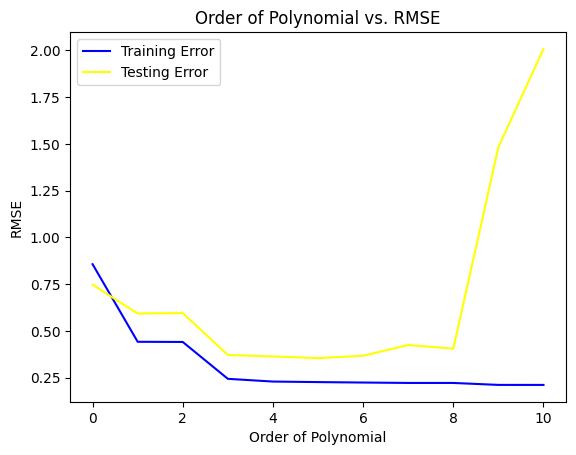
\includegraphics[width=0.8\textwidth]{RMSE.png}
  \caption{The Order of the Polynomial vs Root Mean Square Error (Go Warriors!)}
\end{figure}


When \( m < 3 \), the model exhibits underfitting, as indicated by a relatively large training error when compared to the test error. The lowest test error is achieved with a 5th-degree polynomial. Underfitting is evident where both test and training errors are high, ranging roughly from 0.75 to 1. As polynomial degree \( m \) increases, adding model complexity, training error steadily falls, whereas test error initially declines before abruptly rising after degree 5, the optimal complexity as previously discussed. This steep increase in test error, alongside low training error for high degrees, signals overfitting. Polynomials of degree 4 to 6 provide the best fit for the data. Beyond \( m > 8 \), we observe overfitting, where the test error significantly rises while training error diminishes.



\end{document}